\documentclass[11pt]{article}
\usepackage[a4paper,margin=2.4cm]{geometry}
\usepackage{amsmath,amssymb}
\usepackage{graphicx}
\usepackage{booktabs}
\usepackage{array}
\usepackage{longtable}
\usepackage{xcolor}
\usepackage[hidelinks]{hyperref}
\usepackage{caption}
\captionsetup{font=small}

\newcommand{\Neff}{N_{\mathrm{eff}}}
\newcommand{\chizero}{\chi_0}

\title{\textbf{The minimal classically conformal non-Abelian model for the NANOGrav signal:\\
a dark $SU(2)_D$ Coleman--Weinberg supercooled first-order phase transition}}
\author{DarkAgents}
\date{2026-06-07}

\begin{document}
\maketitle

\begin{abstract}
We report a research-level analysis of \texttt{su2cw-dark}, the minimal classically scale-invariant
non-Abelian dark-sector model proposed to explain the NANOGrav~15\,yr stochastic gravitational-wave
(GW) signal. The model is a dark $SU(2)_D$ gauge theory with a single complex scalar doublet, no
fermions, and Coleman--Weinberg (CW) radiative symmetry breaking. A strongly supercooled first-order
phase transition (FOPT) generates a nano-Hertz GW background. Using a semianalytic CW + high-$T$
backend we computed the FOPT thermodynamics; using a dissipative-bulk-flow (dbf) spectral template
and a PTArcade NG15 Bayesian campaign we fitted the signal, obtaining a posterior peaked at
$g\simeq0.87$ and $\chizero\simeq1.1\,$GeV (MAP), with a best benchmark scoring 14/14 PTA frequency
bins. The decisive limitation, retained by explicit user choice, is that the minimal \emph{secluded}
model has no Standard-Model (SM) portal: thermal equilibrium ($\xi=1$) is assumed but cannot be
realized without a portal, leaving the binding BBN reheating and $\Delta\Neff$ constraints
undetermined and the cosmological viability conditional. We answer the user's question affirmatively
at the level of the GW fit, while flagging the secluded-portal/BBN--$\Neff$ tension and the
template/prior dependence of the preferred region as the controlling caveats.
\end{abstract}

\section{Prompt}
The original user request, verbatim:
\begin{quote}
\textit{``what is the minimal conformal non-abelian model that can explain the NANOGrav signal?''}
\end{quote}
Branch: \texttt{fopt-pta}. The user explicitly elected to keep the minimal secluded model despite the
constraint stage flagging a BBN/$\Neff$ portal tension; this report presents that tension
transparently as the key limitation rather than resolving it.

\section{Summary}
The minimal conformal non-Abelian candidate is a classically scale-invariant dark $SU(2)_D$ gauge
sector with a single complex scalar doublet and CW dimensional transmutation (model
\texttt{su2cw-dark}). It reproduces the NANOGrav~15\,yr signal through a supercooled FOPT whose GW
spectrum is modelled with the dbf template~\cite{LewickiVaskonen2025}. The PTArcade NG15 posterior
prefers $g=0.883\pm0.035$ and $\log_{10}(\chizero/\mathrm{GeV})=-0.051\pm0.173$ (MAP
$g=0.866$, $\chizero=1.12\,$GeV). The model class is not novel: it is essentially that of
Borah--Dasgupta--Kang~\cite{Borah2021}, applied here to the 15\,yr data set. The dominant open issue
is the absence of a SM portal, which makes the binding BBN and $\Delta\Neff$ constraints
non-evaluable and is known to strongly disfavour a strictly secluded dark-sector FOPT~\cite{Bringmann2023}.

\section{Model description}
\label{sec:model}
This section follows the validated output of the \texttt{critic-agent} (handoff
\texttt{handoff\_model.json}, status \texttt{ok}, no red flags).

\paragraph{Field content and symmetries.}
The gauge group is a dark non-Abelian $SU(2)_D$ with coupling $g$. The matter content is a single
complex scalar doublet $\Phi$ (fundamental of $SU(2)_D$, 4 real degrees of freedom). There are no
fermions. The Lagrangian possesses classical scale (conformal) invariance: no dimensionful parameter
appears. An accidental custodial $SO(4)\simeq SU(2)\times SU(2)$ of the single-doublet quartic is
present but not gauged.

\paragraph{Lagrangian.}
\begin{equation}
\mathcal{L} = (D_\mu\Phi)^\dagger (D^\mu\Phi) - \tfrac14 W^a_{\mu\nu}W^{a\,\mu\nu}
- \lambda\,(\Phi^\dagger\Phi)^2 ,
\qquad
D_\mu\Phi = \big(\partial_\mu - i g \tfrac{\sigma^a}{2} W^a_\mu\big)\Phi ,
\end{equation}
with $a=1,2,3$. The potential is a pure quartic; classical scale invariance forbids any $\mu^2
\Phi^\dagger\Phi$ mass term.

\paragraph{Coleman--Weinberg breaking and spectrum.}
Scale invariance is broken radiatively by dimensional transmutation. In unitary gauge
$\Phi=\tfrac{1}{\sqrt2}(0,\chi)^T$ with $\langle\chi\rangle=\chizero$; the doublet vev fully breaks
$SU(2)_D\to\text{nothing}$ (3 Goldstones eaten). The physical states are three degenerate massive dark
gauge bosons $W_D$ (9 dof) and one radial CW pseudo-dilaton $\chi$ (1 dof). The field-dependent masses
are
\begin{equation}
m_W^2(\chi)=\frac{g^2\chi^2}{4},\qquad m_\chi^2 = \beta_\lambda\,\chizero^2,\qquad
\beta_\lambda=\frac{9\,(g/2)^4 + g_{b,\mathrm{scalar}}^4}{8\pi^2}>0 ,
\end{equation}
so $m_W=g\chizero/2$ and $m_\chi=\sqrt{\beta_\lambda}\,\chizero$. Since bosons dominate,
$\beta_\lambda>0$ is guaranteed, ensuring radiative breaking and a positive $m_\chi^2$.

\paragraph{Parameters.} The two independent parameters are the gauge coupling $g\in[0.3,1.5]$ and the
symmetry-breaking scale $\chizero\in[10^{-4},10^2]\,$GeV. The quartic $\lambda$, $\beta_\lambda$,
$g_{b,\mathrm{scalar}}=\sqrt{\beta_\lambda}$ and $m_\chi$ are dependent (CW-fixed). Fixed:
$n_W=9$, scalar dof $=1$, no fermions. The single-field, mass$\,\propto\,$one-vev structure matches
exactly the \texttt{semianalytic\_pipeline} domain of validity.

\paragraph{Stated model assumptions.} (i) The dark sector is in thermal equilibrium with the SM bath
($\xi=1$); (ii) no fermions, so $\beta_\lambda>0$; (iii) perturbativity $g\lesssim1.5$; (iv) a single
radial background direction. Assumption (i) is later identified as foundationally problematic
(Sec.~\ref{sec:assumptions}).

\section{Pipeline status}
\label{sec:status}
Table~\ref{tab:status} records the status of each stage. Two downstream stages (constraints, prior
audit) carry \texttt{warning} status, driven by the unresolved secluded-portal issue; their warnings
are pipeline limitations, not failures.

\begin{table}[h]
\centering
\small
\begin{tabular}{@{}llp{8.4cm}@{}}
\toprule
Stage / handoff & Status & Note \\
\midrule
\texttt{handoff\_model.json} (critic) & ok & Validated, no red flags, no fixes. \\
\texttt{handoff\_critique.json} & warning & Branch-viability flags (completion; broad $\chizero$; high-$T$). \\
\texttt{handoff\_librarian\_preliminary.json} & ok & 4 verified papers; model \emph{not novel}. \\
\texttt{handoff\_fopt.json} & ok & 271/302 viable; 168 in PTA band; percolation verified. \\
\texttt{handoff\_pta.json} & ok & dbf 14/14; PTArcade NG15 posterior obtained. \\
\texttt{handoff\_constraints.json} & warning & Binding BBN/$\Neff$ non-evaluable; portal missing. \\
\texttt{handoff\_prior\_audit.json} & warning & 18 items; secluded-portal gating issue (A01). \\
\bottomrule
\end{tabular}
\caption{Pipeline status by stage.}
\label{tab:status}
\end{table}

\section{Preliminary literature search}
\label{sec:lit}
The \texttt{preliminary-librarian-agent} (status \texttt{ok}) returned four verified papers and a
\emph{not novel} verdict. The \texttt{su2cw-dark} structure is essentially that of
Ref.~\cite{Borah2021} (same $SU(2)_D$ + doublet + CW + supercooled sub-GeV FOPT), which already fitted
NANOGrav 12.5\,yr; the conformal/supercooled idea has been extended to 15\,yr in closely related
Abelian $U(1)'$ models~\cite{Balan2025,Goncalves2025}. The $SU(2)$+doublet+CW structure itself is
established at the electroweak scale~\cite{Mohamadnejad2020} (mHz LISA band, \emph{not} PTA).

\begin{table}[h]
\centering
\small
\begin{tabular}{@{}lp{4.0cm}p{6.4cm}@{}}
\toprule
arXiv & Class & Benchmark hint / role \\
\midrule
2109.11558~\cite{Borah2021} & same model & $g_D=1.37$; $M_{Z_D}\sim0.8$--$8$\,MeV; $\alpha\sim0.4$; $\beta/H\sim140$--$150$. Direct anchor (12.5\,yr). \\
2502.19478~\cite{Balan2025} & structurally similar ($U(1)'$+fermions) & 15\,yr target; extreme supercooling: $\alpha\sim10^3$--$10^7$, $\beta/H\sim18$--$34$, vev $\mathcal{O}(0.1$--$1)$\,GeV. \\
2501.11619~\cite{Goncalves2025} & same signal, $U(1)'$ & Confirms supercooling/completion subtleties (metadata only). \\
1907.08899~\cite{Mohamadnejad2020} & structurally similar (EW scale) & Methodology only; mHz band, benchmarks not PTA-usable. \\
\bottomrule
\end{tabular}
\caption{Verified literature anchors. Convention: $m_W=g\chizero/2$ ($SU(2)$) vs $m_{A'}=gv$
($U(1)'$).}
\label{tab:lit}
\end{table}

\noindent The librarian flagged theory uncertainties: transition completion in deep supercooling, the
high-$T$ expansion validity, and the renormalization-scale dependence of the CW potential.

\section{FOPT results}
\label{sec:fopt}
The \texttt{fopt-agent} (status \texttt{ok}) executed the \texttt{semianalytic\_pipeline} (one-loop CW +
high-$T$ thermal potential). The scan produced 302 points, of which 271 are viable and 168 lie in the
PTA band; all viable points percolate (percolation temperature $T_p$ finite,
\texttt{eternal\_inflation}=False). We define $\alpha$ (transition strength), $\beta/H$ (inverse
duration), $T_n,T_p,T_{\rm reh}$ (nucleation, percolation, reheating temperatures), and $f_{\rm
peak}^{\rm est}$ (a template-independent order-of-magnitude redshifted peak frequency, \emph{not} the
true spectral peak; the spectrum is owned by the PTA stage).

\begin{table}[h]
\centering
\small
\begin{tabular}{@{}lcccccc@{}}
\toprule
Benchmark & $g$ & $\chizero$ [GeV] & $\alpha$ & $\beta/H$ & $T_{\rm reh}$ [GeV] & $f_{\rm peak}^{\rm est}$ [Hz] \\
\midrule
lit\_anchor\_S1 & 1.37 & $1.20\!\times\!10^{-2}$ & 15.0 & 144 & $1.53\!\times\!10^{-3}$ & $2.7\!\times\!10^{-8}$ \\
best\_1 & 1.30 & $5.34\!\times\!10^{-3}$ & 33.1 & 126 & $6.55\!\times\!10^{-4}$ & $9.9\!\times\!10^{-9}$ \\
best\_2 & 1.15 & $1.23\!\times\!10^{-2}$ & 931 & 62.1 & $1.34\!\times\!10^{-3}$ & $9.9\!\times\!10^{-9}$ \\
best\_3 & 1.45 & $3.51\!\times\!10^{-3}$ & 6.22 & 163 & $4.93\!\times\!10^{-4}$ & $9.6\!\times\!10^{-9}$ \\
best\_4 & 1.40 & $4.48\!\times\!10^{-3}$ & 10.4 & 148 & $5.97\!\times\!10^{-4}$ & $1.1\!\times\!10^{-8}$ \\
best\_5 & 1.25 & $8.11\!\times\!10^{-3}$ & 72.5 & 96.8 & $9.46\!\times\!10^{-4}$ & $1.1\!\times\!10^{-8}$ \\
\bottomrule
\end{tabular}
\caption{FOPT benchmarks (\texttt{handoff\_fopt.json}). All points: \texttt{viable},
\texttt{eternal\_inflation}=False. The temperature convention key is $T_{\rm reh}$.}
\label{tab:fopt}
\end{table}

\paragraph{Diagnostics and caveats.} Of 302 points, 31 failed. Transition completion was checked
explicitly via $T_p$ and the eternal-inflation flag. The reported $\alpha$ grows rapidly toward small
$\chizero$/large $g$ (deep supercooling). Backend caveats: high-$T$ (small field$/T$) expansion;
renormalization scale fixed at $\chizero$; no RG running or daisy resummation; Gaussian percolation
approximation.

\section{PTA results}
\label{sec:pta}
The \texttt{pta-agent} (status \texttt{ok}) produced both a benchmark comparison and a full PTArcade
NG15 Bayesian campaign. No \texttt{pta\_report.md} was written; the narrative below is drawn from
\texttt{handoff\_pta.json} and \texttt{ptarcade\_bayes.json}.

\paragraph{Template choice and validity.}
The GW spectrum is computed with the dissipative-bulk-flow (\textbf{dbf}) template of
Ref.~\cite{LewickiVaskonen2025}, with efficiency $k_{\rm sw}=1$ and relativistic/runaway walls
$v_w\to1$. The model is strongly supercooled with vacuum-energy domination and $\alpha\gg1$, so the
sound-wave/higgsless template (validated only for $\alpha\lesssim0.5$~\cite{Caprini2024Higgsless}) is
excluded; dbf is the physically appropriate choice. \emph{Caveat:} viable PTA-matching points have
$\alpha\sim10^5$ to $>10^{15}$, far above the displayed range of Ref.~\cite{LewickiVaskonen2025}; the
amplitude relation is extrapolated and justified by saturation $K_{\rm sw}=\alpha/(1+\alpha)\to1$.

\paragraph{Benchmark comparison.}
The benchmark scan (672 points, 654 viable) was matched against the 14 NANOGrav PTA violin windows.
After extending $\chizero$ upward to $[10^{-3},10]\,$GeV, 29 points scored the full 14/14. The dbf
template is valid (best score 14/14); higgsless is invalid. The four best-fit points
(Table~\ref{tab:pta}) cluster at $g\sim0.85$--$1.05$, $\chizero\sim0.40$--$1.58\,$GeV.

\begin{table}[h]
\centering
\small
\begin{tabular}{@{}llccccc@{}}
\toprule
Rank & Name & $g$ & $\chizero$ [GeV] & $\alpha$ & $\beta/H$ & $T_\star$ [GeV] \\
\midrule
1 & bench\_lo\_g  & 0.85 & 1.000 & $2.12\!\times\!10^{15}$ & 13.1 & 0.0869 \\
2 & bench\_hi\_chi & 0.85 & 1.585 & $4.62\!\times\!10^{15}$ & 12.6 & 0.1378 \\
3 & bench\_lo\_chi & 0.90 & 0.398 & $1.81\!\times\!10^{11}$ & 18.4 & 0.0366 \\
4 & bench\_hi\_g  & 1.05 & 0.501 & $2.23\!\times\!10^{5}$  & 35.1 & 0.0479 \\
\bottomrule
\end{tabular}
\caption{PTA best-fit benchmarks (\texttt{handoff\_pta.json}); all score 14/14 bins.}
\label{tab:pta}
\end{table}

\paragraph{PTArcade campaign.}
A full PTArcade NG15 \texttt{ceffyl} campaign ($N_{\rm samples}=10^5$) was run with priors
$g\sim\mathrm{Uniform}(0.5,1.5)$ and $\log_{10}(\chizero/\mathrm{GeV})\sim\mathrm{Uniform}(-2,2)$, both
substantially wider than the 14/14 window. Chains are finite; posterior peaks and $3\sigma$ regions
fall well inside the priors. Bayesian estimates:
\begin{equation}
g = 0.883\pm0.035,\qquad \log_{10}(\chizero/\mathrm{GeV}) = -0.051\pm0.173,
\end{equation}
with MAP $g=0.866$, $\chizero=1.12\,$GeV. Credible intervals for $g$:
$[0.852,0.916]$ ($1\sigma$), $[0.845,0.980]$ ($2\sigma$), $[0.843,1.059]$ ($3\sigma$);
for $\log_{10}\chizero$: $[-0.218,0.108]$, $[-0.485,0.184]$, $[-0.837,0.228]$ respectively. At the
$1\sigma$ region the derived masses are $m_W\simeq0.26$--$0.59\,$GeV and $m_\chi\simeq37$--$91\,$MeV
(so $m_\chi<m_W$, and $\chi\to W_D W_D$ is kinematically closed throughout). No evidence/Bayes factor
was computed (no SMBHB model comparison).

\begin{figure}[h]
\centering
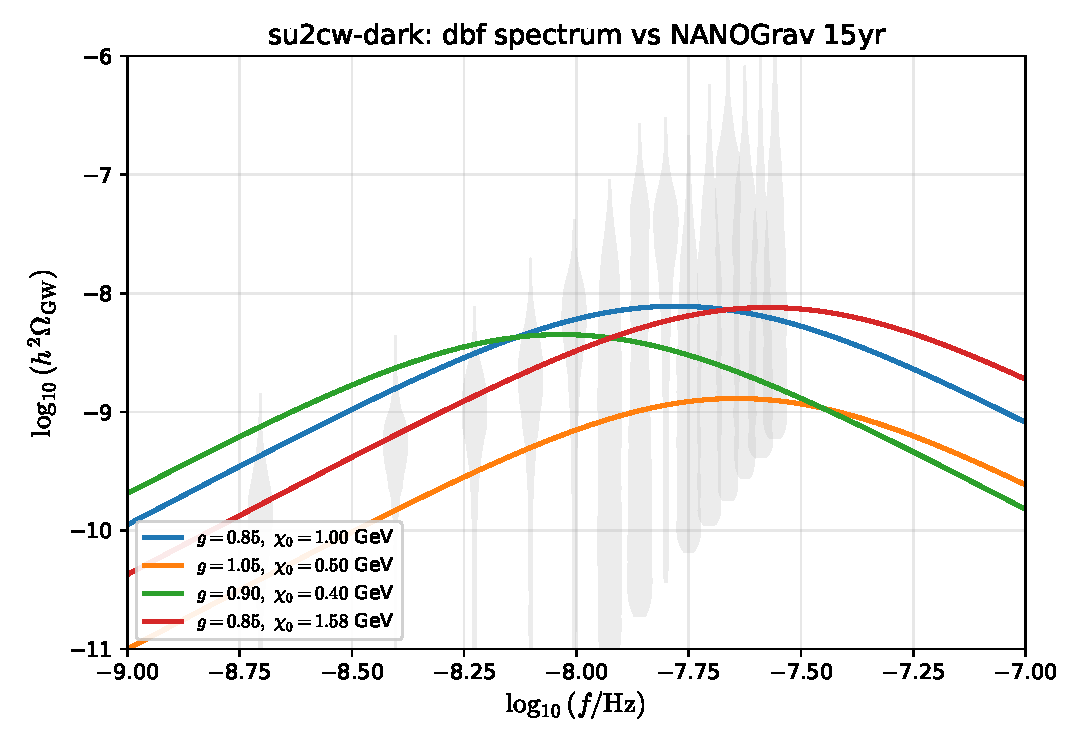
\includegraphics[width=0.78\textwidth]{pta_benchmark_spectrum.pdf}
\caption{GW energy density spectrum $h^2\Omega_{\rm GW}(f)$ versus frequency for the estimated
benchmark point, overlaid on the NANOGrav PTA violins. Source: \texttt{pta\_benchmark\_spectrum.pdf}.}
\label{fig:benchspec}
\end{figure}

\begin{figure}[h]
\centering
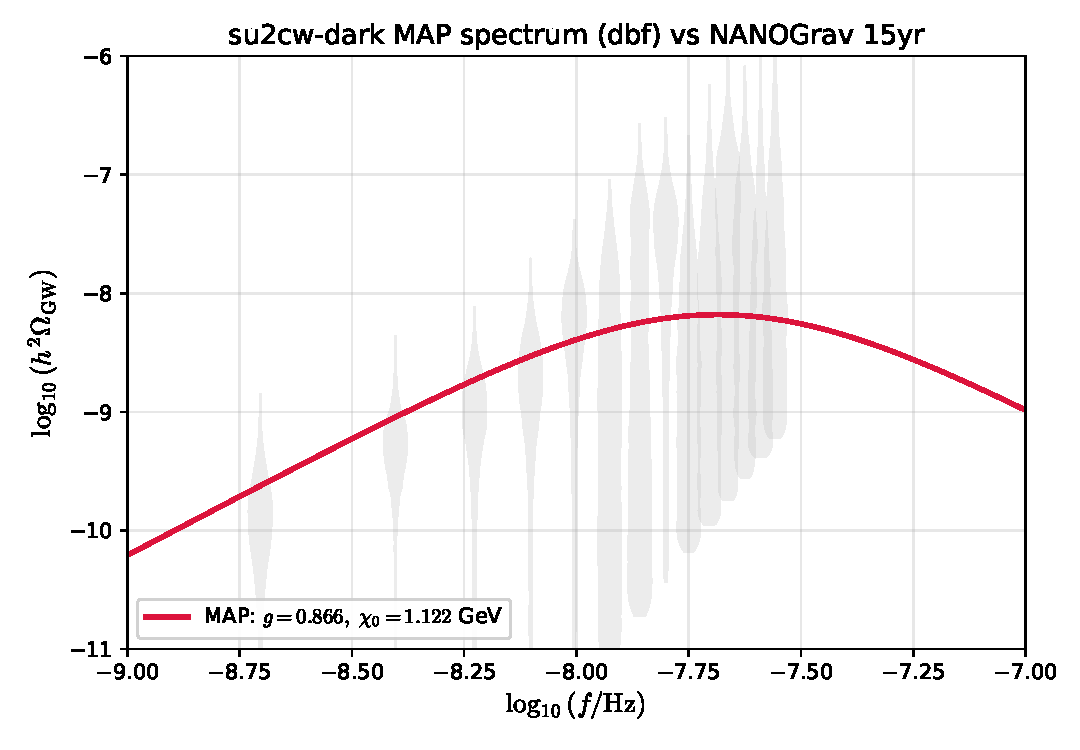
\includegraphics[width=0.78\textwidth]{pta_ptarcade_spectrum.pdf}
\caption{GW spectrum for the PTArcade Bayesian MAP point ($g=0.866$, $\chizero=1.12\,$GeV) versus
frequency, overlaid on the PTA violins. Source: \texttt{pta\_ptarcade\_spectrum.pdf}.}
\label{fig:ptaspec}
\end{figure}

\begin{figure}[h]
\centering
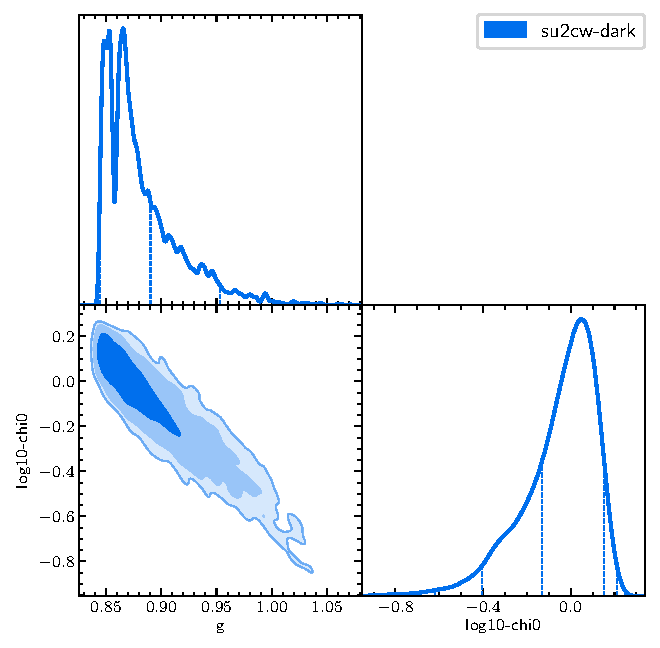
\includegraphics[width=0.7\textwidth]{pta_posteriors.pdf}
\caption{Bayesian posterior distributions in $(g,\log_{10}\chizero)$ from the PTArcade NG15
\texttt{ceffyl} campaign. Source: \texttt{pta\_posteriors.pdf}.}
\label{fig:post}
\end{figure}

\section{Constraints}
\label{sec:constraints}
The \texttt{constraint-agent} (status \texttt{warning}) evaluated 11 constraints on the PTArcade
$1\sigma$ region. The central finding, recorded as a warning, is structural: the model is
\emph{secluded} (no tree-level kinetic-mixing or Higgs portal) yet assumes thermal equilibrium
($\xi=1$). Equilibrium requires a portal; kinetic mixing is forbidden in pure non-Abelian $SU(2)_D$,
and a Higgs portal $|\Phi|^2|H|^2$ breaks the classical conformal invariance the CW mechanism relies
on. This unresolved portal question controls almost every cosmological constraint. Only the theory
self-consistency check (C4, completion) is directly satisfied; the binding cosmological bounds
(C1, C2) cannot be declared pass/fail because the SM-bath reheating and $\Delta\Neff$ are not computed
in any upstream handoff.

\begin{table}[h]
\centering
\small
\begin{tabular}{@{}llp{6.0cm}l@{}}
\toprule
ID & Constraint & Status / role & Source \\
\midrule
C1 & BBN reheating bound & approximate; \emph{not applied} -- binding but SM-bath $T$ not computed & \cite{Bai2021,deSalas2015} \\
C2 & Dark radiation $\Delta\Neff$ & new backend; secluded sector strongly disfavoured & \cite{Bringmann2023} \\
C3 & Portal / thermalization & new backend; foundational, model under-specified & \cite{Balan2025} \\
C4 & FOPT completion/percolation & approximate; \textbf{satisfied} upstream & \cite{Goncalves2025} \\
C5 & Vector DM relic ($W_D$) & new backend; needs portal & \cite{Borah2021} \\
C6 & Pseudo-dilaton $\chi$ stability/late decay & new backend; $m_\chi<m_W$ so $\chi\to W_DW_D$ closed & \cite{Balan2025} \\
C7 & Beam-dump (kinetic mixing) & recast; conditional on portal & \cite{BeamDump2025} \\
C8 & SN1987A cooling & recast; conditional on portal & \cite{Kazanas2014} \\
C9 & Direct detection (sub-GeV) & not applicable (secluded) & \cite{Balan2025} \\
C10 & DM self-interaction (SIDM) & new backend; inputs available, $\sigma/m$ uncomputed & \cite{TulinYu2018}$^{\dagger}$ \\
C11 & Higgs-portal collider & recast; conflicts with conformal invariance & ATLAS/CMS$^{\dagger}$ \\
\bottomrule
\end{tabular}
\caption{Constraints (\texttt{handoff\_constraints.json}). Totals: directly testable 0, approximately
testable 2, requires recast 3, requires new backend 5, not applicable 1.
$^{\dagger}$Source unverified (see Sec.~\ref{sec:refnote}); cited only as descriptive context, not as a
verified literature claim.}
\label{tab:constraints}
\end{table}

\paragraph{Missing backend calculations.} High-priority: (i) SM-bath reheating temperature after
percolation and dark$\to$SM energy transfer (for C1, C2); (ii) dark-to-SM temperature ratio $\xi(T)$
and $\Delta\Neff$ at BBN/CMB (C2, C6); (iii) the portal operator/coupling and thermalization rate
$\Gamma_{\rm portal}/H$ (gates C1--C3, C5--C9, C11); (iv) $W_D$ relic abundance and lifetime (C5).
Medium priority: $\chi$ decay width/abundance (C6) and $W_D$ self-interaction $\sigma/m$ (C10).

\section{Assumptions and limitations}
\label{sec:assumptions}
The \texttt{prior-agent} (status \texttt{warning}) catalogued 18 items. The highest-severity items are
summarized in Table~\ref{tab:assump}. The single decisive limitation is A01, the missing SM portal,
retained by explicit user choice.

\begin{table}[h]
\centering
\small
\begin{tabular}{@{}llcp{6.6cm}@{}}
\toprule
ID & Category & Sev. & Description (controlled?) \\
\midrule
A01 & portal & 9 & No SM portal in a secluded model that nonetheless assumes $\xi=1$; gates BBN, $\Neff$, relic. (no) \\
A02 & BBN & 8 & SM-bath reheating $T$ never computed; pass/fail of BBN bound undetermined. (no) \\
A07 & $\Neff$ & 8 & $\Delta\Neff$ from secluded sector uncomputed; secluded FOPT strongly disfavoured~\cite{Bringmann2023}. (no) \\
A03 & prior/template & 7 & Preferred region template/prior dependent: FOPT center $\chizero\!\sim\!5$\,MeV, $g\!\sim\!1.3$ vs PTA $\chizero\!\sim\!1$\,GeV, $g\!\sim\!0.87$. (no) \\
A04 & GW template & 7 & dbf amplitude extrapolated many orders in $\alpha$; rests on saturation argument. (no) \\
A06 & thermalization & 7 & $\xi=1$ used upstream is inconsistent without a portal; propagates into $\alpha,\beta/H,T_{\rm reh}$. (no) \\
A08 & late decay & 6 & $\chi$ stability/late decays unresolved ($m_\chi<m_W$). (no) \\
A09 & dark matter & 6 & $W_D$ relic abundance uncomputed. (no) \\
A10 & eff. potential & 6 & High-$T$ expansion least accurate exactly in deep supercooling. (yes) \\
A13 & model comparison & 6 & No Bayes factor vs SMBHB; good fit $\neq$ preference over astrophysical background. (no) \\
A12 & statistics/PTA & 5 & PTArcade \texttt{ceffyl} free-spectrum likelihood, not full per-pulsar HD analysis. (yes) \\
A18 & novelty & 3 & Not novel (cf.~\cite{Borah2021}); literature anchor (modest $\alpha$, MeV vev) not reproduced one-to-one. (yes) \\
\bottomrule
\end{tabular}
\caption{Top assumptions/limitations (\texttt{handoff\_prior\_audit.json}); severity 1--10.}
\label{tab:assump}
\end{table}

\paragraph{Critical vs major.} \emph{Critical} (uncontrolled, gate cosmological viability): A01, A02,
A07 (portal/BBN/$\Neff$). \emph{Major limiting} (uncontrolled, affect the preferred region and the
strength of the claim): A03, A04, A06, A08, A09, A13. \emph{Controlled} approximations: A05, A10, A11,
A12, A16, A17, A18.

\section{Reference-verification note}
\label{sec:refnote}
All four primary references were validated against arXiv/INSPIRE-HEP and match the intended title,
authors and content: \texttt{2109.11558}~\cite{Borah2021}, \texttt{2502.19478}~\cite{Balan2025},
\texttt{2511.15687}~\cite{LewickiVaskonen2025} and \texttt{2306.09411}~\cite{Bringmann2023}. One
metadata correction was applied: \texttt{2306.09411} authors are \emph{T.~Bringmann, P.~F.~Depta,
T.~Konstandin, K.~Schmidt-Hoberg, C.~Tasillo} (the constraints handoff listed
``Bringmann, Depta, Hufnagel, Kersten, Mariotti'', which is incorrect); the verified author list is
used here. The handoff source \texttt{2511.15687} (template) is by M.~Lewicki and V.~Vaskonen, ``Impact
of cosmic expansion on gravitational wave spectra from strongly supercooled first-order phase
transitions''. Two constraint-table sources are \emph{unverified} in the upstream handoff
(C10 ``Tulin--Yu'' with \texttt{arxiv\_id} 1705.02358 marked \texttt{citation\_verified:false}, and the
C11 ATLAS/CMS entry with no arXiv ID); they are cited only as descriptive context and are flagged as
unverified in \texttt{handoff\_report.json}. The C7 beam-dump (2507.11163) and C8 SN1987A (1410.0221)
entries are marked verified upstream but were not independently re-validated here; they are reported as
upstream-verified.

\section{Conclusions}
\label{sec:conclusions}
\textbf{Answer to the prompt.} The minimal conformal non-Abelian model that can explain the NANOGrav
signal is a classically scale-invariant dark $SU(2)_D$ gauge theory with one complex scalar doublet
and no fermions, in which CW dimensional transmutation triggers a strongly supercooled first-order
phase transition. With the dbf GW template, this model fits the NANOGrav~15\,yr free spectrum: the
PTArcade NG15 posterior peaks at $g\simeq0.87$, $\chizero\simeq1.1\,$GeV (MAP), and the best benchmark
matches all 14 PTA frequency bins.

\textbf{Robust.} The FOPT thermodynamics and percolation (271/302 viable, completion verified) and the
quality of the dbf spectral fit (14/14 bins; well-constrained posterior inside wide priors) are robust
at the level of the adopted backend and template.

\textbf{Conditional.} The preferred $(g,\chizero)$ region is conditional on the dbf template (with an
amplitude extrapolation across many decades of $\alpha$) and the adopted priors; the FOPT-stage and
PTA-stage preferred corners differ (A03, A04, A18).

\textbf{Blocked / uncontrolled.} The cosmological viability is \emph{not} established. The minimal
model is secluded and has no SM portal, yet equilibrium ($\xi=1$) was assumed. The binding BBN
reheating (C1/A02) and $\Delta\Neff$ (C2/A07) constraints are non-evaluable without computing the
SM-bath reheating and the dark-to-SM energy transfer, and a completely secluded dark-sector FOPT is
\emph{strongly disfavoured}~\cite{Bringmann2023}. Resolving this requires a portal, but kinetic mixing
is forbidden in pure $SU(2)_D$ and a Higgs portal breaks the conformal invariance underpinning the CW
mechanism. \emph{Per the user's explicit choice, the minimal secluded model is retained and this
BBN/$\Neff$ portal tension is reported as the key open limitation rather than patched.} No Bayesian
comparison against the astrophysical SMBHB background was performed (A13), so a good fit does not by
itself establish preference over the standard interpretation.

\textbf{Outlook.} The decisive next step is a model-level portal decision followed by computation of the
SM-bath reheating, $\Delta\Neff$, the $W_D$ relic abundance and $\chi$ lifetime; validation of the dbf
template in the extreme-$\alpha$ regime; a robustness test of the preferred region under alternative
templates/priors and reconciliation with the modest-$\alpha$, MeV-vev anchor of Ref.~\cite{Borah2021};
and a Bayes-factor comparison against the SMBHB interpretation.

\begin{thebibliography}{9}
\bibitem{Borah2021} D.~Borah, A.~Dasgupta, S.~K.~Kang,
\textit{A first order dark $SU(2)_D$ phase transition with vector dark matter in the light of NANOGrav
12.5 yr data}, JCAP \textbf{12} (2021) 039, arXiv:2109.11558.
\bibitem{Balan2025} S.~Balan, T.~Bringmann, F.~Kahlhoefer, J.~Matuszak, C.~Tasillo,
\textit{Sub-GeV dark matter and nano-Hertz gravitational waves from a classically conformal dark
sector}, JCAP \textbf{08} (2025) 062, arXiv:2502.19478.
\bibitem{Goncalves2025} J.~Goncalves, D.~Marfatia, A.~P.~Morais, R.~Pasechnik,
\textit{Supercooled phase transitions in conformal dark sectors explain NANOGrav data}, Phys.\ Lett.\
B \textbf{869} (2025) 139829, arXiv:2501.11619.
\bibitem{Mohamadnejad2020} A.~Mohamadnejad,
\textit{Gravitational waves from scale-invariant vector dark matter model: Probing below the
neutrino-floor}, Eur.\ Phys.\ J.\ C \textbf{80} (2020) 197, arXiv:1907.08899.
\bibitem{LewickiVaskonen2025} M.~Lewicki, V.~Vaskonen,
\textit{Impact of cosmic expansion on gravitational wave spectra from strongly supercooled first-order
phase transitions}, arXiv:2511.15687.
\bibitem{Bringmann2023} T.~Bringmann, P.~F.~Depta, T.~Konstandin, K.~Schmidt-Hoberg, C.~Tasillo,
\textit{Does NANOGrav observe a dark sector phase transition?}, JCAP \textbf{11} (2023) 053,
arXiv:2306.09411.
\bibitem{Bai2021} Y.~Bai, M.~Korwar,
\textit{Cosmological constraints on first-order phase transitions}, arXiv:2109.14765.
\bibitem{deSalas2015} P.~F.~de Salas et al.,
\textit{Bounds on very low reheating scenarios after Planck}, Phys.\ Rev.\ D \textbf{92} (2015)
123534, arXiv:1511.00672.
\bibitem{Caprini2024Higgsless} (Higgsless / sound-wave template validity, $\alpha\lesssim0.5$),
arXiv:2209.04369 (upstream-cited).
\bibitem{BeamDump2025} Beam-dump / dark-photon kinetic-mixing compilation (upstream-cited),
arXiv:2507.11163.
\bibitem{Kazanas2014} D.~Kazanas, R.~N.~Mohapatra, S.~Nussinov, V.~L.~Teplitz, Y.~Zhang,
\textit{Supernova bounds on the dark photon using its electromagnetic decay}, arXiv:1410.0221
(upstream-verified).
\bibitem{TulinYu2018} S.~Tulin, H.-B.~Yu,
\textit{Dark matter self-interactions and small scale structure} (upstream entry \texttt{1705.02358},
\emph{unverified}; cited as context only).
\end{thebibliography}

\end{document}
